\section{Timer/Counter}

\subsection{Timer/Counter Basics}

\begin{minipage}{0.54\linewidth}
\begin{concept}{Timer/Counter Fundamentals}\\
A timer/counter is a digital circuit that counts events:
\begin{itemize}
    \item \textbf{Timer}: Counts clock cycles or processor cycles (periodic)
    \item \textbf{Counter}: Counts external events or signals
\end{itemize}
Common applications:
\begin{itemize}
    \item Triggering periodic software tasks (e.g., display refresh)
    \item Sampling inputs (e.g., buttons) at regular intervals
    \item Counting pulses on an input pin
    \item Measuring time between events
    \item Generating pulse sequences on output pins
\end{itemize}
\end{concept}

\begin{definition}{Timer/Counter Structure}\\
Basic components of a timer/counter system:
\begin{itemize}
    \item \textbf{Counter Register}: 16-bit or 32-bit counter that increments/decrements
    \item \textbf{Prescaler}: Divides input clock to extend counting range
    \item \textbf{Auto-Reload Register (ARR)}: Sets upper limit for counting
    \item \textbf{Source Selection}: Internal clocks, input pins, other timers
    \item \textbf{Control Logic}: Configures counting mode and operation
    \item \textbf{Interrupt Flags}: Signal events to the CPU
\end{itemize}
\end{definition}
\end{minipage}
\begin{minipage}{0.42\linewidth}
\begin{concept}{Counter Modes}\\
\textbf{Up-counting mode}:
\begin{itemize}
    \item Counter starts from 0
    \item Increments up to auto-reload value (ARR)
    \item Generates overflow event when reaching ARR
    \item Resets to 0 and continues
\end{itemize}
\textbf{Down-counting mode}:
\begin{itemize}
    \item Counter starts from auto-reload value (ARR)
    \item Decrements down to 0
    \item Generates underflow event when reaching 0
    \item Reloads ARR value and continues
\end{itemize}
\textbf{Center-aligned mode}:
\begin{itemize}
    \item Counter counts from 0 to ARR-1, then back to 1
    \item Generates events at both up and down counting
    \item Useful for symmetric PWM generation
\end{itemize}
\end{concept}
\end{minipage}


\begin{formula}{Timer Period Calculation}

\begin{minipage}{0.5\linewidth}
For a given timer frequency, the period is calculated as:
$$
T_{timer} = \frac{1}{f_{timer}} 
$$

Timer frequency is derived from the system clock:
$$
f_{timer} = \frac{f_{system}}{(PSC+1)}
$$
\end{minipage}
\hspace{2mm}
\begin{minipage}{0.4\linewidth}
For a desired output frequency:
$$ARR = \frac{f_{timer}}{f_{desired}} - 1$$

For a desired time period:
$$
ARR = f_{timer} \times T_{desired} - 1$$
\end{minipage}
\end{formula}

\begin{example}
Calculate the prescaler (PSC) and auto-reload (ARR) values to generate a 50ms timer period using a 84MHz clock.
\tcblower
We need to find PSC and ARR values to generate a 50ms (0.05s) period.
\vspace{1mm}\\
\begin{minipage}{0.5\linewidth}
Step 1: Choose an appropriate prescaler value.\\
Let's pick a prescaler to generate a 1MHz timer clock:\\
PSC = 84MHz / 1MHz - 1 = 84 - 1 = 83
\vspace{1mm}\\
Step 2: Calculate the auto-reload value.\\
ARR = f\_{timer} × T\_{desired} - 1\\
ARR = 1MHz × 0.05s - 1\\
ARR = 50,000 - 1 = 49,999
\end{minipage}
\hspace{4mm}
\begin{minipage}{0.4\linewidth}
However, this exceeds the 16-bit range \\(maximum 65,535).\\
Let's adjust to use a 10kHz timer clock:\\
PSC = 84MHz / 10kHz - 1 \\ = 8,400 - 1 = 8,399\\
ARR = 10kHz × 0.05s - 1 = 500 - 1 = 499
\vspace{1mm}\\
Therefore:\\
PSC = 8,399,
ARR = 499
\end{minipage}
\end{example}


\begin{definition}{Input Capture}
Input capture is used to measure the timing of external events:
\begin{itemize}
    \item Captures the timer counter value when an event occurs on an input pin
    \item Events can be rising edge, falling edge, or both
    \item Useful for measuring pulse width, period, frequency, or phase difference
    \item Each capture channel has its own register (CCRx)
\end{itemize}
Applications:
\begin{itemize}
    \item Measuring pulse width (e.g., from sensors)
    \item Measuring frequency of input signals
    \item Timing between events
\end{itemize}
\end{definition}



\subsubsection{PWM (Pulse Width Modulation)}

\mult{2}



\begin{definition}{PWM Basics}\\
Pulse Width Modulation is a technique to create analog-like signals using digital outputs:
\begin{itemize}
    \item Signal alternates between high and low state
    \item Fixed frequency (period)
    \item Variable duty cycle (ratio of high time to period)
    \item The average voltage is proportional to duty cycle
\end{itemize}
Applications:
\begin{itemize}
    \item LED dimming
    \item Motor speed control
    \item Digital-to-analog conversion
    \item Signal generation
\end{itemize}
\end{definition}


\begin{concept}{PWM Generation Using Output Compare}\\
Implement PWM using output compare function:
\begin{itemize}
    \item Counter continuously runs through defined range (0 to ARR)
    \item Output pin toggles when counter matches the capture/compare value (CCR)
    \item In up-counting PWM mode 1:
    \begin{itemize}
        \item Output active when counter < CCR
        \item Output inactive when counter $\geq$ CCR
    \end{itemize}
    \item Duty cycle controlled by changing CCR value
\end{itemize}
\end{concept}

\begin{theorem}{PWM Terminology}
\begin{itemize}
    \item \textbf{Period} (T): Time for one complete cycle
    \item \textbf{Frequency} (f): \\ Number of cycles per second (f = 1/T)
    \item \textbf{Duty Cycle} (D): \\ Ratio of high time to period (D = T\_{high}/T)
    \item \textbf{Resolution}: min. change in duty cycle possible
\end{itemize}
\end{theorem}


\begin{concept}{PWM Alignment Types}

\textbf{Edge-aligned PWM}:
    \begin{itemize}
        \item One edge of the pulse is fixed, the other is modulated
        \item Up-counting mode: Leading edge fixed, trailing edge modulated
        \item Down-counting mode: Trailing edge fixed, leading edge modulated
    \end{itemize}
\textbf{Center-aligned PWM}:
    \begin{itemize}
        \item Center of pulse is fixed, both edges are modulated
        \item Produces less harmonic distortion in motor control applications
        \item Implemented using up/down counting mode
    \end{itemize}
\end{concept}


\begin{corollary}{PWM Duty Cycle Calculation}\\
\textbf{Up-counting mode}:
$$
\text{Duty Cycle} = \frac{CCR}{ARR+1} \times 100\%
$$

\textbf{Down-counting mode}:
$$
\text{Duty Cycle} = \left(1 - \frac{CCR}{ARR+1}\right) \times 100\%
$$

\textbf{To achieve a specific duty cycle}:
$$
\text{CCR (up-counting)} = (ARR+1) \times \frac{\text{Duty Cycle}}{100\%} 
$$
$$
\text{CCR (down-counting)} = (ARR+1) \times (1 - \frac{\text{Duty Cycle}}{100\%})
$$
\end{corollary}

\multend

\mult{2}

\begin{example2}{PWM mit 25\% Duty Cycle}\\
    Timer 4 als Upcounter, TIM4\_ARR = 0x9C3F (40000-1)
    
    Gesucht: CCR-Wert für 25\% Duty Cycle mit PWM Mode 1
    
    \tcblower
    
    \textbf{Berechnung:}
    \begin{itemize}
        \item TIMx\_CNT zählt von 0...39999 = 40000 Ticks
        \item Duty Cycle 25\% entspricht 10000 Ticks
        \item PWM Mode 1: OCxREF = '1' solange TIMx\_CNT $<$ TIMx\_CCR
        \item TIM4\_CCR1 = 0x2710 (10000)
    \end{itemize}
    
    \textbf{Downcounter mit PWM Mode 2:}
    Für identisches Signal bei Downcounter/PWM Mode 2:
    \begin{itemize}
        \item PWM Mode 2: OCxREF = '1' solange TIMx\_CNT $>$ TIMx\_CCR
        \item Für 25\% High: CCR = 30000-1 = 0x752F
        \item 39999...30000 = 10000 Ticks High
        \item 29999...0 = 30000 Ticks Low
    \end{itemize}
\end{example2}

\begin{remark}
    Bei PWM-Signalen ist es wichtig zu verstehen, dass die ARR den gesamten Zählbereich definiert (und damit die Periode), während CCR den Umschaltpunkt definiert (und damit den Duty Cycle). Die PWM-Modi bestimmen, wann das Signal High bzw. Low ist.
\end{remark}

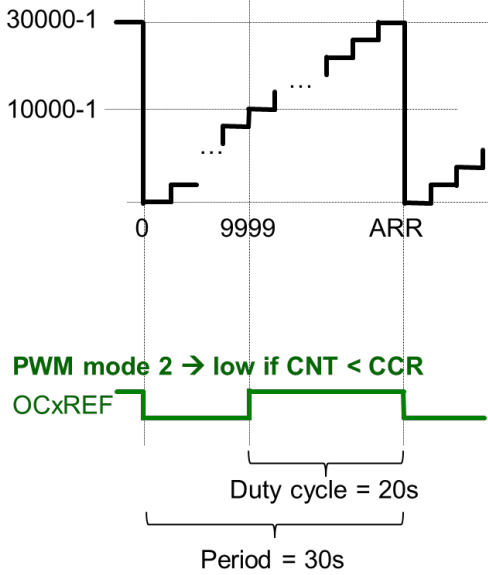
\includegraphics[width=\linewidth]{pmw_signals_ex.png}



\multend

\subsection{Timer Capture/Compare Timing Analysis}

\begin{KR}{Timer-Komponenten verstehen}
    \paragraph{Prescaler}
    \begin{itemize}
        \item Funktionalität: Divisor für Eingangssignal
        \item Zweck: Es wird nur jeder n-te Wert gezählt
        \item Erweitert den Zählbereich des Timers
    \end{itemize}
    
    \paragraph{Counter}
    \begin{itemize}
        \item Funktionalität: Aktueller Timerwert
        \item Zweck: Wird mit jedem n-ten Tick um eins erhöht/erniedrigt
        \item Kann up- oder down-counting sein
    \end{itemize}
    
    \paragraph{Auto Reload Register (ARR)}
    \begin{itemize}
        \item Upcounter: Timer zählt bis zu diesem Wert, dann Überlauf
        \item Downcounter: Startwert für Timer
        \item Definiert die Periode des Timers
    \end{itemize}
    
    \paragraph{Capture/Compare Register (CCR)}
    \begin{itemize}
        \item Capture: Bei einem Event wird Counterwert hier gespeichert
        \item Compare: Event/Interrupt wird ausgelöst, wenn Counter diesen Wert erreicht
        \item Für PWM: Definiert Duty Cycle
    \end{itemize}
\end{KR}

\begin{example2}{Timer-Funktionen}\\
    Timer als Upcounter, Prescaler auf 4 (Register = 0x03), Capture bei steigender Flanke.
    
    \tcblower
    
    \textbf{Capture-Funktion:}
    Bei einem Event wird der Inhalt des Counter Registers in das Capture/Compare Register kopiert. Der Counter läuft weiter.
    
    \textbf{Compare-Funktion:}
    Sobald der Counter den Wert des Capture/Compare Registers erreicht hat, wird ein Event oder Interrupt ausgelöst. Der Counter läuft weiter.
    
    \textbf{Timing-Diagramm:}
    \begin{itemize}
        \item Prescaler teilt durch 4: nur jeder 4. Puls wird gezählt
        \item Bei Event wird aktueller Counter-Wert (z.B. 0x0003) in CCR gespeichert
        \item Counter läuft nach Capture weiter
    \end{itemize}
    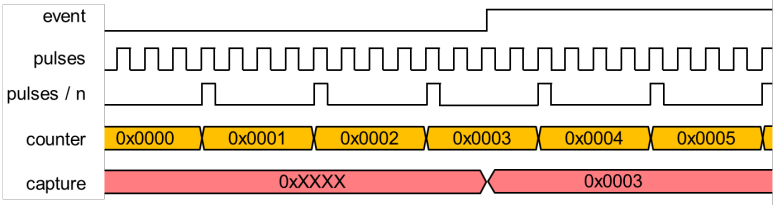
\includegraphics[width=\linewidth]{counter_timer_ex.png}
\end{example2}

\begin{KR}{Analyzing Timer Signal Generation}
\paragraph{Understand the timing diagram}
\begin{itemize}
    \item Identify the timer mode (up-counting, down-counting)
    \item Note the prescaler value and input frequency
    \item Observe the event signals and their timing
\end{itemize}

\paragraph{Trace the counter value}
\begin{itemize}
    \item Start with initial counter value
    \item For up-counting: Increment counter for each clock tick after prescaler
    \item For down-counting: Decrement counter for each clock tick after prescaler
    \item Reset counter when overflow/underflow occurs
    \item Note when capture events occur
\end{itemize}

\paragraph{Analyze capture/compare events}
\begin{itemize}
    \item For capture mode: Counter value is stored in CCRx when event occurs
    \item For compare mode: Compare event occurs when CNT = CCRx
    \item Note the timing of interrupt flags (CCIF)
\end{itemize}

\paragraph{Calculate timing parameters}
\begin{itemize}
    \item Actual period = (ARR+1) × (PSC+1) / timer\_clock
    \item Duty cycle = time\_active / period × 100\%
    \item For PWM: Duty cycle = CCRx / (ARR+1) × 100\% (up-counting mode)
\end{itemize}
\end{KR}

\begin{example2}{Timer Signal Analysis Example}\\
Analyze the following timer configuration:
\begin{itemize}
    \item Timer is configured as up-counter
    \item Source frequency is 0.5 MHz
    \item Prescaler (PSC) = 0x01F3 (499)
    \item Auto-reload (ARR) = 0x752F (30000-1)
    \item Compare value (CCR1) = 0x2710 (10000)
    \item CCMR1 = 0x0070 (PWM Mode 2)
\end{itemize}
Determine the period and duty cycle of the generated PWM signal.

\paragraph{Solution:}
First, calculate the effective counter frequency:
\begin{itemize}
    \item Timer input = 0.5 MHz
    \item Prescaler = 499+1 = 500
    \item Counter frequency = 0.5 MHz / 500 = 1 kHz
\end{itemize}

Calculate the period:
\begin{itemize}
    \item ARR = 30000-1 = 29999
    \item Period = (ARR+1) / counter frequency = 30000 / 1000 Hz = 30 seconds
\end{itemize}

Determine the duty cycle:
\begin{itemize}
    \item PWM Mode 2 means output is active when CNT > CCR1
    \item In up-counting mode, this means output is active when 10000 < CNT $\leq$ 29999
    \item Active time = (29999+1 - 10000) / 1000 Hz = 20 seconds
    \item Duty cycle = Active time / Period = 20s / 30s = 66.67\%
\end{itemize}

Therefore, the PWM signal has:
\begin{itemize}
    \item Period: 30 seconds
    \item Duty cycle: 66.67\% (active for 20 seconds, inactive for 10 seconds)
\end{itemize}
\end{example2}




\raggedcolumns
\columnbreak






\subsection{STM32F4 Timers/Counters}

\mult{2}

\begin{concept}{STM32F4 Timer Types}

\textbf{Basic Timers} (TIM6, TIM7):
    \begin{itemize}
        \item 16-bit counter, prescaler, auto-reload
        \item Simplest timers, mainly for time-base generation
    \end{itemize}
    \textbf{General-Purpose Timers} \small{(TIM2-TIM5, TIM9-TIM14):}
    \normalsize
    \begin{itemize}
        \item TIM2, TIM5: 32-bit timers
        \item TIM3, TIM4: 16-bit timers
        \item Multiple capture/compare channels
        \item Input capture, output compare, PWM generation
    \end{itemize}
    \textbf{Advanced-Control Timers} (TIM1, TIM8):
    \begin{itemize}
        \item Advanced PWM features
        \item Complementary outputs with dead-time insertion
        \item Break input for motor control safety
    \end{itemize}
\end{concept}

\begin{theorem}{Timer Clock Sources}
\begin{itemize}
    \item \textbf{Internal Clock (CK\_INT)}: Default source, derived from system clock
    \item \textbf{External Clock Mode 1}: Timer clock from external pins (TIMx\_CH1, TIMx\_CH2)
    \item \textbf{External Clock Mode 2}: Timer clock from external trigger input (TIMx\_ETR)
    \item \textbf{Internal Trigger Inputs (ITRx)}: Using one timer as prescaler for another
\end{itemize}
\end{theorem}

\begin{corollary}{Key Timer Registers}\\
Important registers for timer configuration:
\begin{itemize}
    \item \textbf{TIMx\_CR1} (Control Register 1):
    \begin{itemize}
        \item CEN: Counter Enable
        \item DIR: Direction (0=up, 1=down)
        \item CMS: Center-aligned Mode Selection
    \end{itemize}
    \item \textbf{TIMx\_PSC} (Prescaler):
    \begin{itemize}
        \item Divides clock frequency by a factor between 1 and 65536
        \item Actual division factor is PSC+1
    \end{itemize}
    \item \textbf{TIMx\_ARR} (Auto-reload Register):
    \begin{itemize}
        \item Sets period in up-counting mode
        \item Sets initial value in down-counting mode
    \end{itemize}
    \item \textbf{TIMx\_CNT} (Counter):
    \begin{itemize}
        \item Current counter value
    \end{itemize}
    \item \textbf{TIMx\_SR} (Status Register):
    \begin{itemize}
        \item UIF: Update Interrupt Flag
        \item CCxIF: Capture/Compare Interrupt Flags
    \end{itemize}
    \item \textbf{TIMx\_DIER} (DMA/Interrupt Enable Register):
    \begin{itemize}
        \item UIE: Update Interrupt Enable
        \item CCxIE: Capture/Compare Interrupt Enable
    \end{itemize}
\end{itemize}
\end{corollary}

\multend

\subsubsection{Timer Configuration}

\begin{concept}{Understanding Timer Configuration}
\begin{itemize}
    \item \textbf{Prescaler (PSC):} Divides input clock frequency by (PSC+1)
    \item \textbf{Counter (CNT):} Current count value
    \item \textbf{Auto-reload register (ARR):} Value to reload after overflow/underflow
    \item \textbf{Update flag (UIF):} Set when counter overflows/underflows
\end{itemize}

\paragraph{Calculate timer parameters}
\begin{itemize}
    \item Determine desired period (T): The time between events
    \item Calculate required counts: counts = T × input\_frequency
    \item If counts > 65,536 (16-bit limit), use prescaler:
    \begin{itemize}
        \item Choose prescaler value (PSC): PSC = PSC = (Clock\_Freq / gewünschte\_Freq) - 1
        \item Adjusted counter value: ARR = ARR = (gewünschte\_Freq / overflow\_Freq) - 1
    \end{itemize}
    \item For precision, minimize prescaler while keeping ARR within limits
\end{itemize}
\end{concept}


\begin{KR}{Timer konfigurieren}
    \paragraph{Clock-Source auswählen}
    \begin{itemize}
        \item TIMx\_SMCR Register: SMS[2:0] = 000 für interne Clock (CK\_INT)
        \item Andere Quellen: externe Pins, andere Timer (siehe Reference Manual)
    \end{itemize}

    \paragraph{Register setzen}
    \begin{itemize}
        \item TIMx\_PSC: Prescaler-Wert
        \item TIMx\_ARR: Auto-Reload-Wert
        \item TIMx\_CR1: Timer-Konfiguration (Up/Down)
        \item Enable interrupt if needed in TIMx\_DIER (UIE bit)
        \item Enable timer by setting CEN bit in TIMx\_CR1
    \end{itemize}
    
    \textbf{Zählrichtung festlegen}:
    \begin{itemize}
        \item TIMx\_CR1 Register: DIR Bit
        \item DIR = 0: Upcounter
        \item DIR = 1: Downcounter
    \end{itemize}
    
    \textbf{Overflow-Zeit berechnen}:
    \begin{itemize}
        \item Gewünschte Zeit und Clock-Frequenz gegeben
        \item Mehrere Kombinationen möglich!
    \end{itemize}
\end{KR}



\begin{example2}{Basic Timer Configuration} to generate an interrupt every 1 second (timer clock frequency is 84 MHz)
\paragraph{Calculations and Setup}
First, calculate the required counts: counts = 1s × 84MHz = 84,000,000
\vspace{1mm}\\
Since 84,000,000 > 65,536 (16-bit limit), we need a prescaler:
\begin{itemize}
    \item Choose prescaler: PSC = 8400 - 1 = 8399
    \item This divides the clock to 84MHz/8400 = 10kHz
    \item Adjusted counter value: ARR = 10,000 - 1 = 9999
\end{itemize}

\paragraph{Configuration Steps}
\textbf{Step 1: Enable timer clock} -
Enable the clock to the timer peripheral using RCC register.

\textbf{Step 2: Configure prescaler} -
Set the prescaler value to divide the timer clock.

\textbf{Step 3: Configure auto-reload value} -
Set period in up-counting mode or initial value in down-counting mode

\textbf{Step 4: Configure counting mode} -
Select up-counting, down-counting, or center-aligned mode.

\textbf{Step 5: Configure interrupts (if needed)} -
Enable update or capture/compare interrupts.

\textbf{Step 6: Enable the timer} -
Set the CEN bit in the CR1 register.

\begin{lstlisting}[language=C, style=basesmol]
// Configure TIM2 for a 1Hz interrupt (1s period)
// Assuming system clock = 84MHz

// Step 1: Enable TIM2 clock
RCC->APB1ENR |= RCC_APB1ENR_TIM2EN;

// Step 2: Configure prescaler
// PSC = (SystemCoreClock / 2) / 10000 - 1
TIM2->PSC = 8399;  // Produces 10kHz timer clock (84MHz/8400)

// Step 3: Configure auto-reload value
// ARR = (timer clock / desired frequency) - 1
TIM2->ARR = 9999;  // 10kHz/10000 = 1Hz

// Step 4: Configure counting mode (up-counting, default)
TIM2->CR1 &= ~TIM_CR1_DIR;  // Up-counting mode

// Step 5: Enable update interrupt
TIM2->DIER |= TIM_DIER_UIE;
// Step 6: Enable timer
TIM2->CR1 |= TIM_CR1_CEN;

// Configure NVIC to handle TIM2 interrupt
NVIC_EnableIRQ(TIM2_IRQn);
NVIC_SetPriority(TIM2_IRQn, 1);
\end{lstlisting}

\begin{itemize}
    \item Timer clock frequency: 84MHz
    \item Prescaler: 8400 (gives 10kHz)
    \item Auto-reload: 10,000 (gives 1Hz)
    \item Timer period: 1 second
\end{itemize}
\end{example2}


\begin{example2}{Timer für 200ms Overflow}
    Timer konfigurieren:
    \begin{itemize}
        \item Source: CK\_INT mit 84 MHz
        \item Upcounter
        \item Overflow alle 200 ms
    \end{itemize}
    
    \textbf{Lösung 1:}
\begin{lstlisting}[style=basesmol]
TIM3_SMCR &= 0xFFF8;     // SMS[2:0] = 000 (CK_INT)
TIM3_CR1 &= 0xFF8F;      // DIR = 0 (Upcounter)
TIM3_PSC = 0x20CF;       // (8400-1) -> 10 kHz
TIM3_ARR = 0x07CF;       // (2000-1) -> 200 ms
\end{lstlisting}
    
    \textbf{Lösung 2:}
\begin{lstlisting}[style=basesmol]
TIM3_PSC = 0x0347;       // (840-1) -> 100 kHz
TIM3_ARR = 0x4E1F;       // (20000-1) -> 200 ms
\end{lstlisting}
    
    \textbf{Berechnung:}
    84 MHz / 8400 = 10 kHz, 10 kHz / 2000 = 5 Hz = 200 ms Periode
\end{example2}

\subsubsection{Input Capture}



\begin{KR}{Input Capture Configuration}
\paragraph{Step 1: Configure GPIO pin}
Configure the GPIO pin as alternate function for the timer channel.
\paragraph{Step 2: Configure timer base}
Set up the timer's prescaler and period.
\paragraph{Step 3: Configure capture channel}
Configure the channel for input capture and set the edge sensitivity.
\paragraph{Step 4: Enable interrupts}
Enable capture interrupt and NVIC if notification is required.
\paragraph{Step 5: Enable timer}
Start the timer counting.

\begin{lstlisting}[language=C, style=basesmol]
// Configure TIM3 Channel 1 for input capture on rising edge

// Step 1: Configure GPIO pin (PA6 for TIM3_CH1)
RCC->AHB1ENR |= RCC_AHB1ENR_GPIOAEN;
GPIOA->MODER &= ~GPIO_MODER_MODER6;
GPIOA->MODER |= GPIO_MODER_MODER6_1;  // Alternate function
GPIOA->AFR[0] &= ~GPIO_AFRL_AFRL6;
GPIOA->AFR[0] |= 2 << GPIO_AFRL_AFRL6_Pos;  // AF2 for TIM3

// Step 2: Configure timer base
RCC->APB1ENR |= RCC_APB1ENR_TIM3EN;
TIM3->PSC = 83;     // 84MHz/84 = 1MHz timer clock
TIM3->ARR = 65535;  // Maximum period

// Step 3: Configure capture channel
// CC1S[1:0] = 01 (input, IC1 mapped to TI1)
TIM3->CCMR1 &= ~TIM_CCMR1_CC1S;
TIM3->CCMR1 |= TIM_CCMR1_CC1S_0;

// Configure input filter and prescaler if needed
TIM3->CCMR1 &= ~(TIM_CCMR1_IC1F | TIM_CCMR1_IC1PSC);

// Configure edge sensitivity (rising edge)
TIM3->CCER &= ~(TIM_CCER_CC1P | TIM_CCER_CC1NP);

// Enable capture
TIM3->CCER |= TIM_CCER_CC1E;

// Step 4: Enable capture interrupt
TIM3->DIER |= TIM_DIER_CC1IE;
NVIC_EnableIRQ(TIM3_IRQn);

// Step 5: Enable timer
TIM3->CR1 |= TIM_CR1_CEN;
\end{lstlisting}
\end{KR}

\subsubsection{PWM Output Configuration}

\begin{concept}{Understanding PWM Output Configuration}
\paragraph{Understand PWM parameters}
\begin{itemize}
    \item \textbf{Period:} Controlled by ARR value
    \item \textbf{Duty cycle:} Controlled by CCRx value
    \item \textbf{Frequency:} Determined by timer clock, prescaler, and ARR
\end{itemize}
Implementation:
\begin{itemize}
        \item PWM Mode 1 (Upcounting): OCxREF = '1' solange TIMx\_CNT $<$ TIMx\_CCR
        \item PWM Mode 2 (Upcounting): OCxREF = '0' solange TIMx\_CNT $<$ TIMx\_CCR
        \item Downcounting: Logik ist invertiert
    \end{itemize}

\paragraph{Calculate PWM parameters}
\begin{itemize}
    \item PWM frequency = Timer clock / ((PSC+1) × (ARR+1))
    \item For up-counting mode:
    \begin{itemize}
        \item CCRx controls when output switches from active to inactive
        \item Duty cycle = CCRx / (ARR+1) × 100\%
    \end{itemize}
    \item For down-counting mode:
    \begin{itemize}
        \item CCRx controls when output switches from inactive to active
        \item Duty cycle = (ARR+1-CCRx) / (ARR+1) × 100\%
    \end{itemize}
\end{itemize}

\textbf{Periode vs. Duty Cycle}
    \begin{itemize}
        \item Periode wird durch ARR bestimmt
        \item Duty Cycle wird durch CCR bestimmt
        \item Frequenz = Timer\_Clock / ((PSC + 1) $\times$ (ARR + 1))
    \end{itemize}

\paragraph{Configure PWM output}
\begin{itemize}
    \item Configure timer basic parameters (PSC, ARR)
    \item Select PWM mode in CCMRx register:
    \begin{itemize}
        \item PWM Mode 1: Output active when CNT < CCRx
        \item PWM Mode 2: Output active when CNT > CCRx
    \end{itemize}
    \item Set CCRx value to control duty cycle
    \item Enable output in CCER register (CCxE bit)
    \item Configure GPIO pin for alternate function (timer output)
    \item Enable timer by setting CEN bit in CR1
\end{itemize}
\textbf{Register konfigurieren}:
    \begin{itemize}
        \item TIMx\_CCMR: OCxM[2:0] = 110 (PWM Mode 1) oder 111 (PWM Mode 2)
        \item TIMx\_CCER: CCxE = 1 (Output Enable)
        \item TIMx\_CCR: Duty Cycle Wert
    \end{itemize}
\end{concept}


\begin{example2}{PWM-Signal aus Registerwerten analysieren}\\
    Gegebene Konfiguration:
    \begin{itemize}
        \item Source: 0.5 MHz
        \item TIM3\_PSC = 0x01F3 (500-1)
        \item TIM3\_ARR = 0x752F (30000-1)
        \item TIM3\_CCR1 = 0x2710 (10000)
        \item TIM3\_CCMR1 = 0x0070 (PWM Mode 2)
    \end{itemize}
    
    \tcblower
    
    \textbf{Analyse:}
    \begin{itemize}
        \item Prescaler: 500-1 $\rightarrow$ 0.5 MHz / 500 = 1 kHz
        \item ARR: 30000-1 $\rightarrow$ Periode \\ = 30000 / 1 kHz = 30 Sekunden
        \item CCR: 10000 $\rightarrow$ 10 Sekunden
        \item PWM Mode 2: Low wenn CNT $<$ CCR
    \end{itemize}
    
    \textbf{Resultat:}
    \begin{itemize}
        \item Periode: 30 Sekunden
        \item Duty Cycle: 20 Sekunden High (30s - 10s)
        \item 0...9999: Low (10s), 10000...29999: High (20s)
    \end{itemize}
\end{example2}


\begin{KR}{PWM Configuration}
\paragraph{Step 1: Configure GPIO pin}
Configure the GPIO pin as alternate function for the timer channel.
\paragraph{Step 2: Configure timer base}
Set prescaler and auto-reload value to define PWM frequency.
\paragraph{Step 3: Configure PWM mode}
Set output compare mode to PWM and configure polarity.
\paragraph{Step 4: Set initial duty cycle}
Write the initial CCR value.
\paragraph{Step 5: Enable output and timer}
Enable output and start the timer.
\end{KR}

\begin{example2}{PWM Configuration} PWM output at 1kHz with 50\% duty cycle

\begin{lstlisting}[language=C, style=basesmol]
// Step 1: Configure GPIO pin (PA6 for TIM3_CH1)
RCC->AHB1ENR |= RCC_AHB1ENR_GPIOAEN;
GPIOA->MODER &= ~GPIO_MODER_MODER6;
GPIOA->MODER |= GPIO_MODER_MODER6_1;  // Alternate function
GPIOA->AFR[0] &= ~GPIO_AFRL_AFRL6;
GPIOA->AFR[0] |= 2 << GPIO_AFRL_AFRL6_Pos;  // AF2 for TIM3

// Step 2: Configure timer base
RCC->APB1ENR |= RCC_APB1ENR_TIM3EN;
TIM3->PSC = 83;    // 84MHz/84 = 1MHz timer clock
TIM3->ARR = 999;   // 1MHz/1000 = 1kHz PWM frequency

// Step 3: Configure PWM mode
// CC1S = 00: Channel configured as output
TIM3->CCMR1 &= ~TIM_CCMR1_CC1S;

// OC1M = 110: PWM mode 1 (active when counter < CCR1)
TIM3->CCMR1 &= ~TIM_CCMR1_OC1M;
TIM3->CCMR1 |= TIM_CCMR1_OC1M_1 | TIM_CCMR1_OC1M_2;

// Enable output compare preload
TIM3->CCMR1 |= TIM_CCMR1_OC1PE;

// Set active high polarity
TIM3->CCER &= ~TIM_CCER_CC1P;

// Step 4: Set initial duty cycle (50%)
TIM3->CCR1 = 500;  // 50% of 1000

// Step 5: Enable output and timer
TIM3->CCER |= TIM_CCER_CC1E;  // Enable output
TIM3->CR1 |= TIM_CR1_CEN;     // Enable counter
\end{lstlisting}
\end{example2}




\begin{example2}{PWM Configuration}
Configure Timer 4 to generate a 20kHz PWM signal with 75\% duty cycle on Channel 2, system clock = 84MHz:\\
1. \textbf{Calculate timer settings for 20kHz:}
\begin{itemize}
    \item Let's use prescaler = 3 (divide by 4)
    \item Timer clock = 84MHz/4 = 21MHz
    \item For 20kHz: ARR = 21MHz/20kHz - 1 = 1049
\end{itemize}
2. \textbf{Calculate CCR value for 75\% duty cycle:}
\begin{itemize}
    \item Up-counting mode, PWM mode 1
    \item CCR = (ARR+1) * 0.75 = 1050 * 0.75 = 787
\end{itemize}
3. \textbf{Configuration code:}
\begin{lstlisting}[language=C, style=basesmol]
// Configure GPIO pin (PB7 for TIM4\_CH2)
RCC->AHB1ENR |= RCC_AHB1ENR_GPIOBEN;
GPIOB->MODER &= ~GPIO_MODER_MODER7;
GPIOB->MODER |= GPIO_MODER_MODER7_1;  // Alternate function
GPIOB->AFR[0] &= ~GPIO_AFRL_AFRL7;
GPIOB->AFR[0] |= 2 << GPIO_AFRL_AFRL7_Pos;  // AF2 for TIM4
// Configure timer base
RCC->APB1ENR |= RCC_APB1ENR_TIM4EN;
TIM4->PSC = 3;     // 84MHz/4 = 21MHz
TIM4->ARR = 1049;  // 21MHz/1050 = 20kHz
// Configure PWM mode
TIM4->CCMR1 &= ~TIM_CCMR1_CC2S;  // Channel as output
TIM4->CCMR1 &= ~TIM_CCMR1_OC2M;
TIM4->CCMR1 |= TIM_CCMR1_OC2M_1 | TIM_CCMR1_OC2M_2;  // PWM mode 1
TIM4->CCMR1 |= TIM_CCMR1_OC2PE;  // Enable preload
TIM4->CCER &= ~TIM_CCER_CC2P;    // Active high
// Set duty cycle (75%)
TIM4->CCR2 = 787;
// Enable output and timer
TIM4->CCER |= TIM_CCER_CC2E;
TIM4->CR1 |= TIM_CR1_CEN;
\end{lstlisting}
\end{example2}



\begin{example2}{PWM Configuration}
Configure Timer 4 for PWM output with: ARR = 0x9C3F (value 39999), Up-counting mode, PWM Mode 1 and 25\% duty cycle
\vspace{1mm}\\
Then, reconfigure for down-counting mode with PWM Mode 2 while maintaining the same electrical signal.
\paragraph{Solution:}
For up-counting mode with PWM Mode 1:
\begin{itemize}
    \item Total count is 40,000 (ARR+1)
    \item For 25\% duty cycle, the output should be high for 10,000 counts
    \item In PWM Mode 1 (up-counting): CCR1 = 25\% of 40,000 = 10,000 = 0x2710
\end{itemize}

For down-counting mode with PWM Mode 2:
\begin{itemize}
    \item In PWM Mode 2 (down-counting), output is active when CNT > CCR1
    \item To maintain 25\% duty cycle: CCR1 = ARR+1-10,000 = 40,000-10,000 = 30,000 = 0x752F
\end{itemize}

C code for configuration:
\begin{lstlisting}[language=C, style=basesmol]
// Up-counting mode, PWM Mode 1, 25% duty cycle
TIM4->ARR = 0x9C3F;       // Auto-reload value (39999)
TIM4->CCR1 = 0x2710;      // Compare value for 25% duty cycle (10000)
TIM4->CCMR1 = 0x0060;     // PWM Mode 1 for channel 1
TIM4->CCER |= 0x0001;     // Enable output for channel 1
TIM4->CR1 &= ~TIM_CR1_DIR; // Up-counting mode
TIM4->CR1 |= TIM_CR1_CEN;  // Enable timer

// Down-counting mode, PWM Mode 2, 25% duty cycle
TIM4->ARR = 0x9C3F;       // Auto-reload value (39999)
TIM4->CCR1 = 0x752F;      // Compare value for 25% duty cycle (30000)
TIM4->CCMR1 = 0x0070;     // PWM Mode 2 for channel 1
TIM4->CCER |= 0x0001;     // Enable output for channel 1
TIM4->CR1 |= TIM_CR1_DIR;  // Down-counting mode
TIM4->CR1 |= TIM_CR1_CEN;  // Enable timer
\end{lstlisting}
\end{example2}





